\documentclass[border=4pt]{standalone}
\usepackage{tikz}
\usetikzlibrary{arrows.meta,calc}

\begin{document}
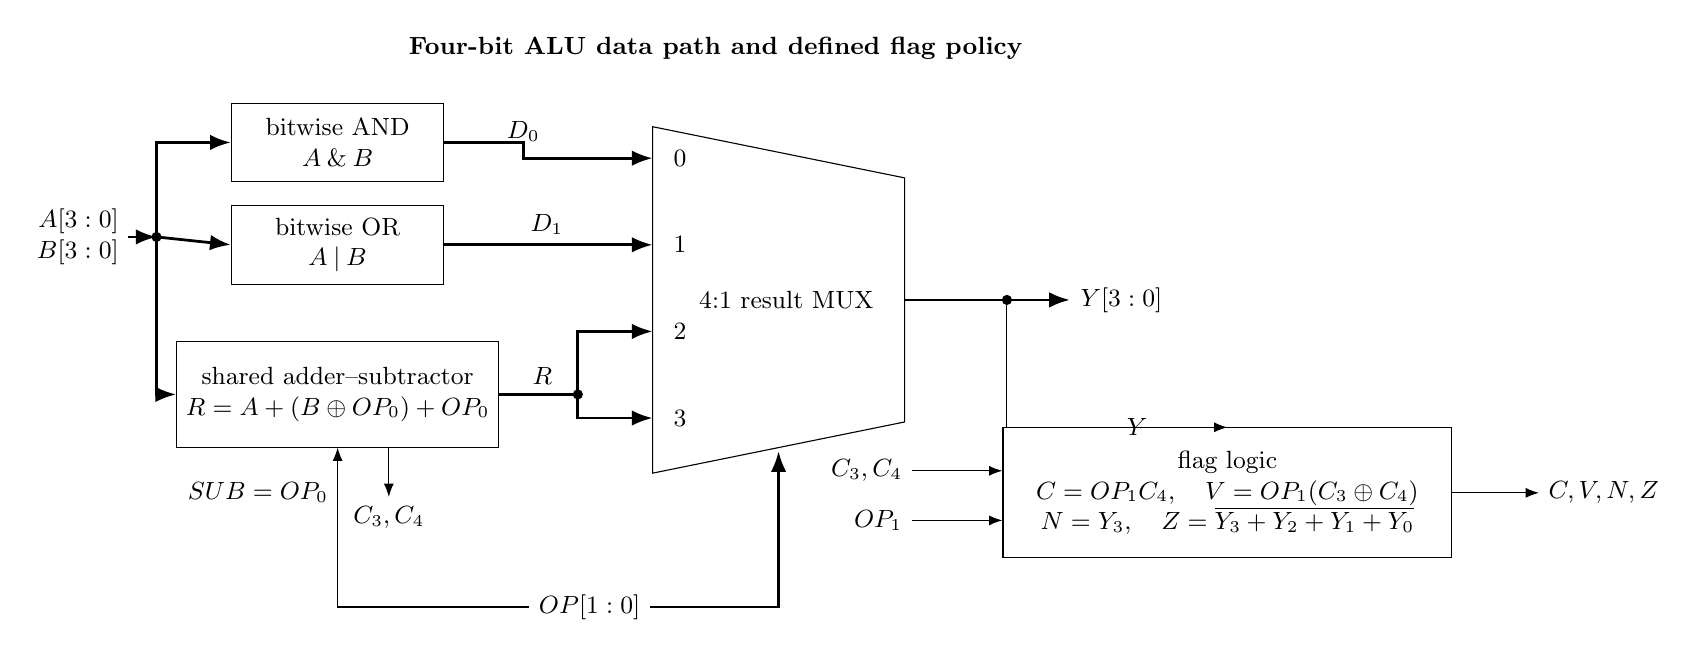
\begin{tikzpicture}[
  >=Latex,
  font=\small,
  block/.style={draw,minimum width=2.7cm,minimum height=1.0cm,align=center},
  bus/.style={->,line width=1.0pt}
]
  \node[font=\small\bfseries] at (8.8,7.2)
    {Four-bit ALU data path and defined flag policy};

  \node[align=right] (AB) at (0.7,4.8) {$A[3:0]$\\$B[3:0]$};
  \node[block] (AND) at (4.0,6.0)
    {bitwise AND\\$A\mathbin{\&}B$};
  \node[block] (OR) at (4.0,4.7)
    {bitwise OR\\$A\mathbin{|}B$};
  \node[block,minimum height=1.35cm] (AS) at (4.0,2.8)
    {shared adder--subtractor\\$R=A+(B\oplus OP_0)+OP_0$};

  \coordinate (FAN) at (1.7,4.8);
  \draw[bus] (AB.east) -- (FAN);
  \node[circle,fill,inner sep=1.3pt] at (FAN) {};
  \draw[bus] (FAN) |- (AND.west);
  \draw[bus] (FAN) -- (OR.west);
  \draw[bus] (FAN) |- (AS.west);

  \draw (8.0,1.8) -- (11.2,2.45) -- (11.2,5.55) -- (8.0,6.2) -- cycle;
  \node at (9.7,4.0) {4:1 result MUX};
  \node at (8.35,5.8) {0};
  \node at (8.35,4.7) {1};
  \node at (8.35,3.6) {2};
  \node at (8.35,2.5) {3};

  \draw[bus] (AND.east) -- ++(1.0,0) |- (8.0,5.8)
    node[pos=0.3,above] {$D_0$};
  \draw[bus] (OR.east) -- ++(1.3,0) |- (8.0,4.7)
    node[pos=0.3,above] {$D_1$};
  \coordinate (RJ) at ($(AS.east)+(1.0,0)$);
  \coordinate (D2) at (8.0,3.6);
  \coordinate (D3) at (8.0,2.5);
  \draw[bus] (AS.east) -- (RJ) -- (RJ |- D2) -- (D2);
  \node[circle,fill,inner sep=1.3pt] at (RJ) {};
  \node[above] at ($(AS.east)!0.55!(RJ)$) {$R$};
  \draw[bus] (RJ) -- (RJ |- D3) -- (D3);

  \node (OP) at (7.2,0.1) {$OP[1:0]$};
  \draw[bus] (OP) -- (9.6,0.1) -- (9.6,2.08);
  \draw[->] (OP.west) -- (4.0,0.1) -- (4.0,2.125)
    node[pos=0.72,left] {$SUB=OP_0$};

  \coordinate (YJ) at (12.5,4.0);
  \draw[bus] (11.2,4.0) -- (YJ) -- ++(0.8,0)
    node[right] {$Y[3:0]$};
  \node[circle,fill,inner sep=1.3pt] at (YJ) {};

  \node[block,minimum width=5.7cm,minimum height=1.65cm] (FLAGS)
    at (15.3,1.55)
    {flag logic\\
     $C=OP_1C_4,\quad V=OP_1(C_3\oplus C_4)$\\
     $N=Y_3,\quad Z=\overline{Y_3+Y_2+Y_1+Y_0}$};

  \draw[->] (YJ) -- (YJ |- FLAGS.north) -- (FLAGS.north)
    node[midway,right] {$Y$};
  \draw[->] ($(AS.south)+(0.65,0)$) -- ++(0,-0.62)
    node[below] {$C_3,C_4$};
  \draw[->] ($(FLAGS.west)+(-1.15,0.28)$)
    node[left] {$C_3,C_4$} -- ($(FLAGS.west)+(0,0.28)$);
  \draw[->] ($(FLAGS.west)+(-1.15,-0.35)$)
    node[left] {$OP_1$} -- ($(FLAGS.west)+(0,-0.35)$);
  \draw[->] (FLAGS.east) -- ++(1.1,0)
    node[right] {$C,V,N,Z$};
\end{tikzpicture}
\end{document}
